\documentclass[../main.tex]{subfiles}

\begin{document}

En este apartado se discutirá el estado en el que se encuentran las tecnologías y las herramientas que abarcan y apoyan el desarrollo de este TFG. También se aportará el conocimiento teórico asociado al desarrollo, obtenido mediante un amplio proceso de investigación bibliográfica.

\section{Geometría no euclidiana}

Durante el desarrollo del proyecto haremos uso de una geometría que no cumple el quinto postulado de Euclides anteriormente mencionado. Para entender mejor qué significa esto y cómo afecta a la sensación de inmersión del usuario, a continuación se describe brevemente la historia de la geometría no euclidiana y algunos ejemplos de su aplicación en videojuegos.

\subsection{Historia de la geometría no euclidiana}

Como se ha explicado antes, la geometría definida por Euclides en el año 300 a.C. fue la única geometría conocida durante siglos.

No es hasta el siglo XVIII que se hacen avances tratando de comprobar si los postulados definidos por Euclides son absolutos o no. Según Coxeter \cite{Coxeter}, Giovanni Gerolamo Saccheri, uno de los principales precursores de la geometría no euclidiana, trató de probar el quinto postulado \cite{Saccheri_GP}, ya que estaba convencido de que la geometría Euclidiana era una verdad absoluta. Después de mucho tiempo de investigación, Saccheri concluyó que el quinto postulado de Euclides era imposible de demostrar, y más tarde, prescindiendo de él, demostró que negándolo se incurre en contradicción. De esta manera nacieron los conceptos de geometría hiperbólica y elíptica, ambas no euclidianas.

Todos estos siglos de investigación que concluyen en que el problema no tiene solución, despertaron el interés de Carl Friederich Gauss, cuyo trabajo llevó al descubrimiento de nuevas geometrías cuyos sistemas estaban liberados del quinto postulado. Gauss fue la primera persona que tuvo una visión clara sobre este tipo de geometría, pero no publicó su investigación. El conocimiento que obtuvo Gauss no se reveló hasta pasados más de treinta años gracias al trabajo de Nikolái Lobachevski \cite{Lobachevski} y János Bolyai \cite{Bolyai}, que tenían ideas muy próximas a las suyas. Tal y como explica Roberto Bonola \cite{Bonola}, todos sustituyeron el quinto postulado de Euclides, llegando a la conclusión de que, dado un punto exterior a una recta A, sin importar su posición, existen infinitas rectas que lo atraviesan sin intersectar con la recta A. También demostraron que la suma de los ángulos de un triángulo es siempre menor que la suma de dos ángulos rectos (180º), y que la suma de estos ángulos es menor cuanto mayor es el área del triángulo.

Con estos nuevos conceptos, se pueden plantear geometrías alternativas que permiten cosas que eran imposibles hasta el momento. Para entender mejor el significado de las investigaciones de Gauss, Lobachevski y Bolyai, se propone un ejemplo en el que se dibujan líneas rectas sobre un cuerpo esférico, tal y como se ve en la figura \ref{fig:Triangle_on_Sphere}.

%%Esfera tridimensional
\begin{figure}[htbp]
\centering
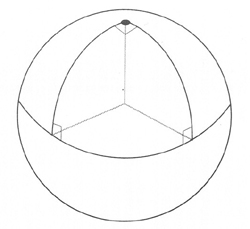
\includegraphics[width= 5cm, height= 4.5cm]{imagenes/Triangle_on_Sphere.jpg}
\caption{Geometría no euclidiana sobre una esfera. Fuente:\cite{Triangle_on_Sphere}}
\label{fig:Triangle_on_Sphere}
\end{figure}

En este ejemplo tenemos dos líneas rectas paralelas que recorren la esfera desde arriba, y otra línea, también recta, que intersecta con ambas horizontalmente, formando así ángulos rectos. Estas tres lineas forman un triángulo y, para poder analizarlo mejor, se estudia esta situación en dos dimensiones, como aparece en la figura \ref{fig:Example_2D}.

%%Ejemplo en 2D
\begin{figure}[htbp]
\centering
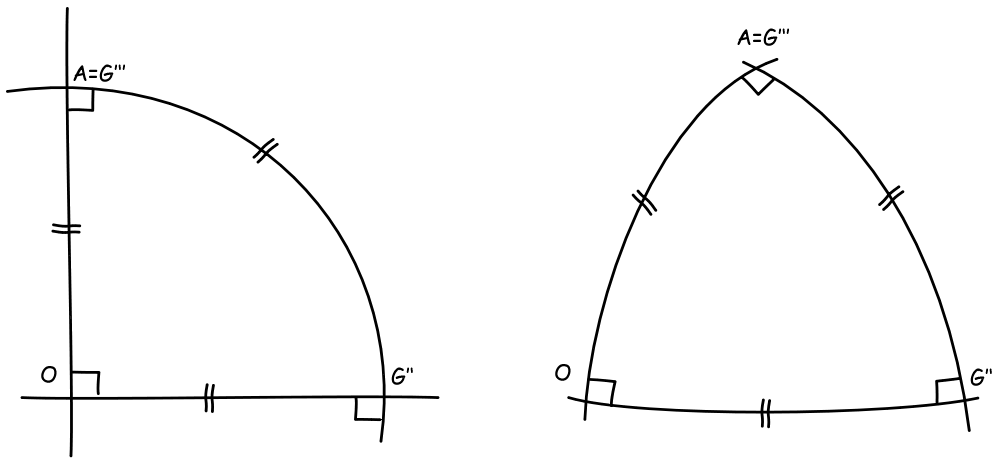
\includegraphics[width= 10cm, height= 5cm]{imagenes/Non_Euclidian_Example_2D.png}
\caption{Geometría no euclidiana explicada en dos dimensiones. Fuente:\cite{Triangle_on_Sphere_2D}}
\label{fig:Example_2D}
\end{figure}

En dos dimensiones, se puede apreciar curvatura en las rectas dibujadas. Esto es porque las líneas se han dibujado sobre una esfera tridimensional, por lo que, al traducirse a un plano bidimensional aparecen estas curvaturas, aunque todas las líneas sean rectas. Por lo tanto, como tenemos tres líneas rectas unidas por tres vértices, el resultado es un triángulo. Como se ha mencionado anteriormente, la línea horizontal corta a las otras dos formando ángulos rectos, y el último ángulo, formado por la intersección de las dos rectas verticales, forman el último ángulo recto. Según estos cálculos, tenemos entonces un triángulo cuya suma de sus ángulos interiores es la suma de tres ángulos rectos (270º), que no es inferior a la suma de dos ángulos rectos (180º), por lo que podemos concluir que tenemos una geometría que no cumple el quinto postulado de Euclides.

\subsection{Percepción espacial en entornos no euclidianos en realidad virtual}

La percepción espacial es la capacidad que tenemos los seres humanos de ser conscientes de la relación entre el espacio que nos rodea y nosotros mismos.

Entendemos por espacio todo aquello que nos rodea, es decir, objetos, elementos e incluso otras personas. Se dice que una persona tiene una buena percepción espacial cuando comprende la disposición del entorno que la rodea y su posición respecto a él, aunque también consiste en comprender la relación de los objetos cuando ocurre un cambio de posición en el espacio. Gracias a ella es posible percibir diferentes tamaños, formas o distancias, y podemos reproducir de forma mental objetos tanto tridimensionales como bidimensionales, además de anti- ciparnos a los cambios que existan en el espacio \cite{Spacial_Perception}.

Las personas están constantemente empleando esta habilidad cognitiva para cualquier situación, como por ejemplo correr, escribir o saltar. Tanto es así, que la mayor parte del tiempo hacemos cálculos casi sin pensar, de manera automática, por ejemplo para no chocar contra un muro o bajar unas escaleras. Esto se debe a que estamos acostumbrados al espacio que nos rodea, y con el tiempo mejoramos nuestra percepción y nos adaptamos.

En entornos virtuales, la percepción espacial de un usuario puede ser distinta a la de un entorno real, ya que hay muchos factores que afectan. Algunos de ellos son el nivel de detalle geométrico, la fluidez de navegación, la calidad de las texturas o la profundidad, y pueden influir en los cálculos que realiza una persona para explorar el entorno \cite{Spacial_Perception_on_Games}.

Hay múltiples investigaciones que estudian el comportamiento de las personas cuando se enfrentan a diferentes situaciones en espacios tridimensionales, tanto euclidianos como no euclidianos. Para ver si la percepción de los usuarios varía cuando se encuentran en espacios no euclidianos, Daniel Rotham y William Warren \cite{Spacial_Perception_non_Euclidean} ponen a prueba las habilidades sensoriales de varias personas propo- niendo explorar un entorno determinado.,  primero sin modificaciones y luego utilizando lo que llaman "\uppercase{A}gujero de gusano".

En esencia, los agujeros de gusano son portales que interconectan zonas distintas del espacio para crear la sensación de entorno no euclidiano (Ver figura \ref{fig:Wormhole}). La idea principal es colocar estos agujeros de gusano estratégicamente para crear efectos como acortar pasillos o conectarlos de distinta forma a como estaban anteriormente, de manera que el usuario experimente el espacio con los portales tras haberlo explorado previamente sin ellos.

El entorno virtual consiste en un laberinto de $11 m^2$ que contiene diferentes objetos en determinados puntos. En el escenario B, el agujero de gusano número 1 acorta un pasillo 6 metros y gira al usuario 90º, y el número 2 acorta otro pasillo 10 metros y rota otros 90º al usuario. Los participantes recorren el entorno en ambos escenarios buscando los distintos objetos con la finalidad de comprobar si detectan las incoherencias de un escenario respecto al otro. Se busca comprobar si los usuarios crean un mapa mental del entorno euclidiano, o en su lugar perciben el espacio de una manera diferente.

Los resultados muestran que, al introducir los portales, la mayoría de usuarios no detecta violaciones radicales en la geometría del entorno, mostrando una gran insensibilidad a los cambios propuestos. Daniel y William concluyen que las personas no construyen un mapa cognitivo euclidiano del espacio de navegación, sino que generan una red de caminos que relacionan distintos lugares del espacio, y que se puede describir como un grafo topológico. Además aprenden longitudes y ángulos determinados que les permiten elegir las rutas más cortas u óptimas.

\begin{figure}[h!]
\centering
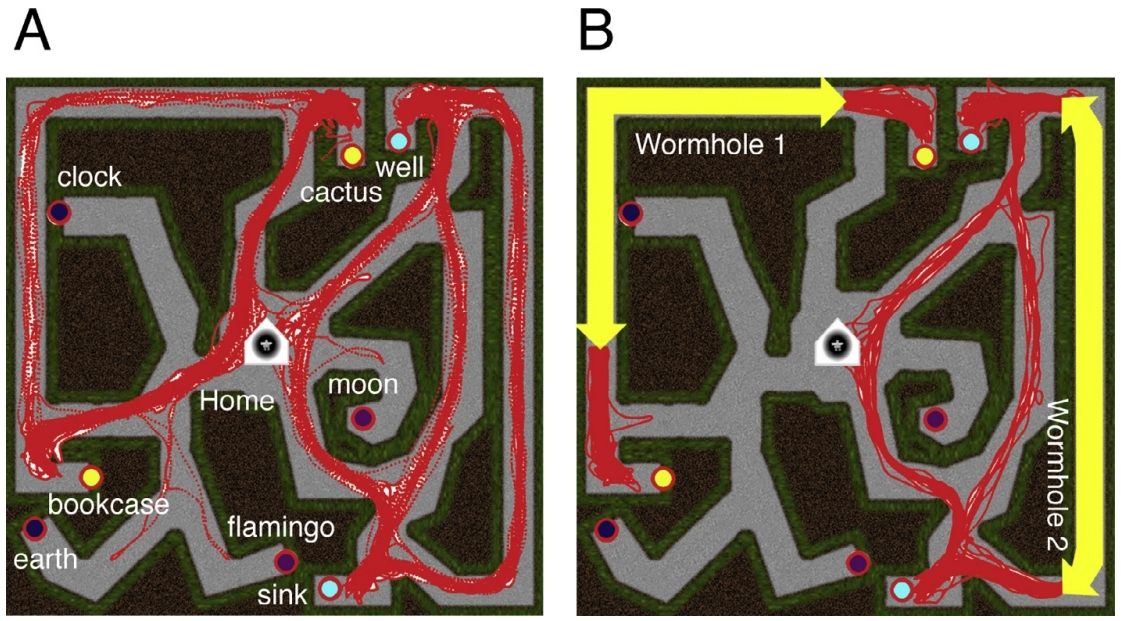
\includegraphics[width=10.5cm, height=5.5cm]{imagenes/Wormholes.jpg}
\caption{Laberinto en realidad virtual. (A) Entorno euclidiano. (B) Entorno no euclidiano. Fuente:\cite{Spacial_Perception_non_Euclidean}}
\label{fig:Wormhole}
\end{figure}

Con toda esta información, se puede concluir que si la percepción espacial de las personas no varía y son capaces de almacenar la información del entorno y sus relaciones, entonces es posible utilizar estas técnicas para generar entornos no euclidianos de manera que sean manejables, controlables e inmersivos.

\subsection{Aplicación de entornos no euclidianos en videojuegos}

El término de entornos no euclidianos en videojuegos era desconocido hasta hace poco tiempo. En los últimos años, algunos desarrolladores han creados videojuegos utilizando este concepto que, en este campo, se reduce a cualquier espacio que no funcione como lo hace el entorno real.

Aunque aún no hay una gran cantidad de videojuegos que apliquen este tipo de entornos, sí que hay algunas personas que lo han investigado, como por ejemplo Vinícius Silva y Tiago Novello \cite{NE_Videogames_3D}, que han creado un sistema inmersivo que permite visualizar espacios no euclidianos utilizando \textit{Ray Tracing}\footnote{El ray tracing o trazado de rayos es un algoritmo para síntesis de imágenes que calcula el camino de la luz como píxeles en un plano de la imagen y simula sus efectos sobre las superficies virtuales en las que incide.} en tiempo real. 

El resultado de su investigación permite a un usuario visualizar algunas estructuras geométricas no euclidianas como los \textit{Manifolds} que son, en esencia, espacios topológicos en los que la distancia de un punto a otro no es necesariamente el segmento que los une, es decir, la distancia euclidiana (Ver figura \ref{fig:Manifold}). De esta forma se pueden observar espacios hiperbólicos tridimensionales que de otra manera no sería posible.

%%Ejemplo de Manifolds
\begin{figure}[htbp]
\centering
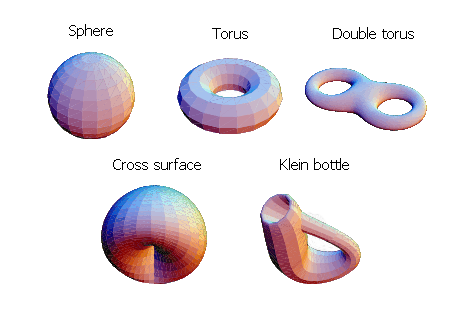
\includegraphics[width= 11cm, height= 8cm]{imagenes/Manifold.png}
\caption{Ejemplo de Manifolds tridimensionales. Fuente:\cite{Manifold}}
\label{fig:Manifold}
\end{figure}

No todos los videojuegos que dicen utilizar entornos no euclidianos, los utilizan. De hecho, hay gran parte de ellos que utilizan algunos trucos y técnicas para simularlos. Un ejemplo sería superponer la geometría de espacios diferentes, lo que permite crear experiencias como \textit{Hyperbolic Maze} \cite{Hyperbolic_Maze} creado por Zeno Rogue.

Con este tipo de efectos se puede hacer que el usuario experiencie situaciones que jamás serían posibles en el mundo real, como por ejemplo rodear una columna y que el espacio cambie a ser otro completamente diferente al que había antes de rodearla, o crear bucles que devuelvan al usuario a un punto determinado del espacio por el que ya ha pasado.

\subsubsection{Antichamber}

Uno de los juegos que más ha influido en el desarrollo de este proyecto es Antichamber.

Antichamber es un juego que contiene espacios imposibles y aún así consigue explicar cómo jugar sin necesidad de tutoriales gracias a una buena gestión del espacio, utilizando pasajes simulados en una estructura en forma de laberinto que el jugador puede explorar \cite{Antichamber}. Este juego utiliza las técnicas que se han comentado anteriormente, de manera que puede conectar espacios diferentes para que, en momentos determinados, el jugador pase de estar en un sitio a otro, tratando de crear sensaciones de bucle o teletransporte. Alexander Bruce, el desarrollador de Antichamber, hace uso de la perspectiva para intentar engañar al usuario y manipularlo.

Las situaciones que se pueden encontrar en este juego son muchas, como por ejemplo pasillos infinitos, o habitaciones en las que nos encontramos aparentemente encerrados, y no hay camino por el que seguir. Uno de los primeros retos que se proponen al empezar Antichamber es el llamado "puzle de las escaleras" (Ver figura \ref{fig:Antichamber_Puzzle}). En él, el jugador se encuentra frente a dos escaleras, una roja y una azul.

%%Puzle de Antichamber
\begin{figure}[htbp]
\centering
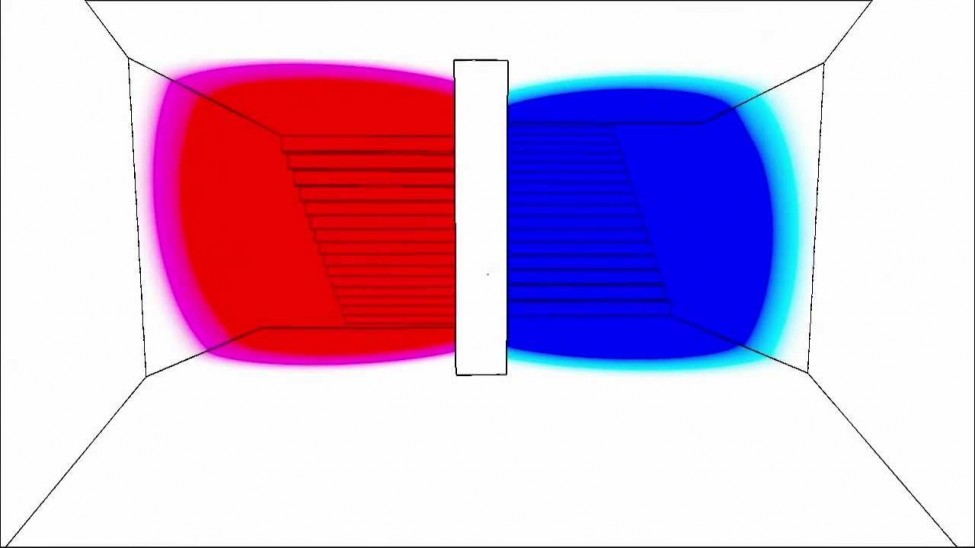
\includegraphics[width= 11cm, height= 8cm]{imagenes/Antichamber_puzzle.jpg}
\caption{Antichamber: Puzle de las escaleras. Fuente:\cite{Antichamber_Puzzle}}
\label{fig:Antichamber_Puzzle}
\end{figure}

En primera instancia, parece que el usuario debe tomar una decisión, tomar las escaleras rojas o las azules pero, en realidad, la decisión que se tome es irrelevante para resolver el acertijo. Tanto si el jugador decide ir por la izquierda como por la derecha, acaba de nuevo frente a las dos escaleras, en a la misma situación. Cuando se toma uno de los caminos, al volver al mismo punto aparece un nuevo letrero que dice "La elección no importa si el resultado es el mismo". La solución final es tomar ambos caminos una vez, y una vez delante de las escaleras, retroceder hacia atrás, donde el jugador encontrará un letrero que dice "\uppercase{C}uando vuelves donde estuviste, las cosas no siempre son como las recordabas", junto a un nuevo camino que permite al usuario continuar con el juego.

Con estas pruebas el desarrollador pone a prueba el ingenio de los jugadores mientras trata de transmitir sus ideas y distintas lecciones de vida.

Este concepto abre infinidad de oportunidades para crear entornos manipulables en los que se tiene el control absoluto, de manera que es posible crear cualquier bucle o camino que fuese necesario y utilizar la perspectiva para engañar al usuario.

\subsubsection{Portal}

Para entender el desarrollo de este proyecto, es de gran interés estudiar Portal, que es uno de sus referentes principales.

Portal es un videojuego de puzles, que basa toda su jugabilidad alrededor de una pistola de portales de la que puede hacer uso el jugador, siendo posible abrir dos portales interconectados en cualquier punto. Para avanzar, el usuario debe hacer frente a diferentes situaciones que debe superar gracias a esta pistola y las plataformas y objetos de las distintas habitaciones.

%%Imágen de Portal el videojuego(3D)
\begin{figure}[htbp]
\centering
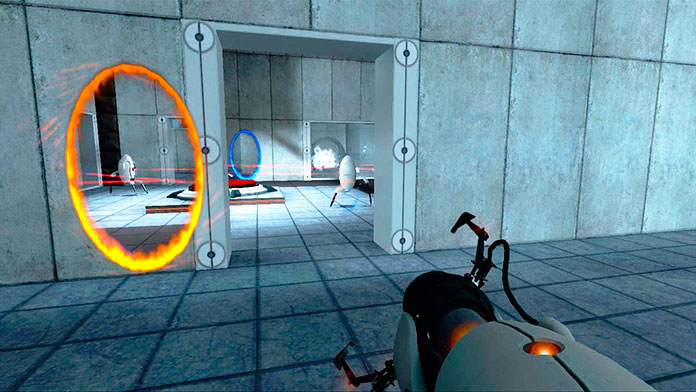
\includegraphics[width= 9cm, height= 6cm]{imagenes/Portal_Game_3D.jpg}
\caption{Captura del videojuego Portal. Fuente:\cite{Portal_Game_3D}}
\label{fig:Portal_Game_3D}
\end{figure}

Este juego, al igual que Antichamber, no utiliza geometría no euclidiana en el diseño de sus niveles, si no que utiliza los portales para superponer unos espacios tridimensionales sobre otros para crear este efecto. Esto es posible gracias a distintas cámaras auxiliares que capturan la posición del jugador relativa a varios puntos, que se proyecta posteriormente sobre planos bidimensionales que son, en esencia, los portales. En la figura \ref{fig:Portal_Game_3D} se puede ver un ejemplo de este concepto ya que se superpone en la habitación actual del usuario (Portal naranja) un fragmento del espacio de la habitación que tiene más adelante (Portal azul).

Para superar los distintos niveles es necesario colocar los portales estratégicamente para poder llegar a sitios que serían imposibles de otra forma. Esto es posible ya que la conexión de los portales trasciende lo visual, pudiendo el usuario atravesar uno de ellos al acercarse lo suficiente y salir por el otro, consiguiendo la sensación de teletransporte.

Además, cuando el jugador atraviesa uno de los portales, conserva toda la inercia y el impulso que tenía inicialmente, lo que abre infinidad de soluciones distintas a los puzles que se proponen. El sentido en el que ejerce la fuerza de gravedad siempre es el mismo y las coordenadas locales del jugador no se rotan al cruzar portales, por lo que es posible, por ejemplo, saltar hacia un portal en el suelo y aparecer en una altura superior manteniendo la velocidad y la inercia que se consiguen gracias a la fuerza de gravedad (Ver figura \ref{fig:Portal_Game_2D}).

Con las funcionalidades que proporcionan estos portales, el videojuego propone multitud de puzles en los que busca poner a prueba la inteligencia, ingenio y percepción espacial de los jugadores, que deben entender casi a la perfección el entorno que les rodea y los objetos que lo componen para poder resolverlos.

La manera en la que se utilizan estos portales, al igual que en  el videojuego Antichamber, permite a los desarrolladores crear entornos sobre los que tienen control absoluto, de manera que es posible utilizarlos para poner a los usuarios en situaciones a las que no están acostumbrados y ver cómo responden.

%%Imágen de Portal el videojuego(2D)
\begin{figure}[htbp]
\centering
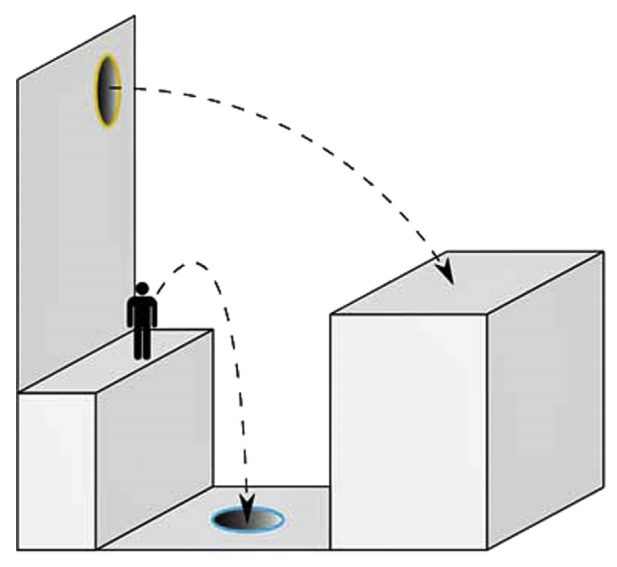
\includegraphics[width= 8cm, height= 7cm]{imagenes/Portal_Game_2D.png}
\caption{Ejemplo de utilización de los portales para subir a una plataforma imposible de alcanzar. Fuente:\cite{Portal_Game_2D}}
\label{fig:Portal_Game_2D}
\end{figure}

Este efecto que consigue Portal es muy similar al efecto del que se hace uso en el desarrollo de este proyecto para conectar distintas habitaciones y, de esta forma, simular espacios no euclidianos

\section{Unity}
Dado que el desarrollo de este trabajo se basa en la realidad virtual, es necesario un motor gráfico que nos proporcione las herramientas necesarias para crear los efectos que nos permitan generar espacios no euclidianos en realidad virtual.

Se define como motor gráfico al framework de software diseñado para crear y desarrollar videojuegos. Todo motor gráfico ha de ofrecer al programador una funcionalidad básica, proporcionando normalmente un motor de renderizado (“render”) para gráficos 2D y 3D, un motor que detecte la colisión física de objetos y la respuesta a dicha colisión, sonidos y música, animación, inteligencia artificial, comunicación con la red para juegos multijugador, posibilidad de ejecución en hilos, gestión de memoria o soporte para localización \cite{Graphic_Engines}.

Para elegir el motor gráfico más adecuado a este trabajo, se tiene en cuenta principalmente las herramientas que proporciona para generar el efecto del portal de manera eficiente y sencilla, y las diferentes facilidades que aporta para desarrollar para ordenador. Una vez evaluados todos estos aspectos, se decide elegir Unity como motor gráfico para la realización del proyecto en su versión 2020.2.0f1 y utilizando su sistema de programación basado en C\#. 

Unity es un motor gráfico multiplataforma que incluye su propio entorno de desarrollo. Principalmente está enfocado al desarrollo de videojuegos, pero puede utilizarse en otros ámbitos que requieran de elementos como renderización en 3D o elementos multimedia. Es uno de los motores gráficos más populares en la actualidad, por lo que hay disponible una gran cantidad de documentación disponible para los desarrolladores. Además, actualmente está en desarrollo su sistema XR, que junta en un sólo término los conceptos de realidad virtual, realidad aumentada y realidad mixta, del que hablaremos más tarde.

\subsection{Elementos básicos de Unity}

Para facilitar el seguimiento y comprensión del desarrollo del proyecto, se exponen brevemente a continuación algunos de los elementos más básicos de Unity que serán necesarios.

\subsubsection{Escenas}

Los videojuegos tienen que acceder a una gran cantidad de información mientras se ejecutan, como personajes, luces, scripts... Toda esta información tiene que estar accesible en todo momento para que se ejecute sin problema. La solución lógica es almacenar todos estos elementos en memoria, pero en proyectos grandes esto podría suponer un problema ya que existe un límite de memoria disponible. Para evitarlo, se estructura el proyecto en distintos niveles, de manera que solo se cargue en memoria la información necesaria en cada momento. Este concepto es conocido en Unity como escena (Ver figura \ref{fig:Escena_Vacía})y cada una de ellas representa un distinto nivel, que al principio en un espacio vacío tridimensional y que podemos utilizar como base para empezar a desarrollar.

%%Imagen de una escena en Unity, centrada y con la referencia a la figura
\begin{figure}[h!]
\centering
\includegraphics[width=9.5cm, height=6cm]{imagenes/Unity_escena_vacía.png}
\caption{Escena vacía en Unity. Fuente:\cite{Scene_Documentation}}
\label{fig:Escena_Vacía}
\end{figure}

\subsubsection{GameObjects}

El GameObject es el concepto más importante en el editor de Unity.

Cada objeto de la escena es un GameObject, desde personajes u objetos hasta luces, cámaras, sistemas de partículas... Sin embargo estos GameObjects no pueden hacer nada por sí mismos, sino que es necesario añadirles componentes y propiedades para que tengan un comportamiento específico. La única propiedad que tienen todos los GameObjects en común es su Transform, que define su posición, rotación y escala dentro de la escena. Esto es así porque los GameObjects de una escena están organizados mediante una jerarquía de tipo árbol, y son emparentados según sus Transform. Por ejemplo, si un GameObject es padre de otro, la propiedad Transform del hijo es relativa a la del padre, y en consecuencia si movemos el transform del padre, también moveremos el del hijo en la misma medida.

Los componentes más importantes que utilizaremos en el proyecto son el Mesh Renderer, que define el material del que están compuestos los objetos tridi- mensionales y permite renderizarlos acorde a como se establezcan sus parámetros, y los Scripts. Estos últimos son, en esencia, el código que permite controlar tanto la escena como el comportamiento de los GameObject, y nos permite instanciarlos desde código y modificar todas sus propiedades.

\subsection{Unity XR} \label{UnityXR_Section}

Unity XR, se basa en el concepto de \textit{eXtended Reality}. Este término se refiere a la combinación de todos los entornos, tanto reales como virtuales, y todas las interacciones, tanto las generadas por ordenador como las que permiten los periféricos.

Existen distintos tipos de sistemas de realidad extendida relacionados entre ellos, y que Unity XR pretende englobar. Dichos sistemas son los siguientes:

\begin{itemize}
    \item \textbf{Realidad virtual(VR):} simulación de un entorno completamente diferente entorno al usuario.
    \item \textbf{Realidad aumentada(AR):} superpone elementos y los muestra al usuario sobre el entorno real.
    \item \textbf{Virtualidad aumentada(AV):}  presenta entornos virtuales cuya interfaz los hace más intuitivos.
    \item \textbf{Realidad mixta(MR):} permite combinar entornos creados con el mundo real.
\end{itemize}

\begin{figure}[h!]
\centering
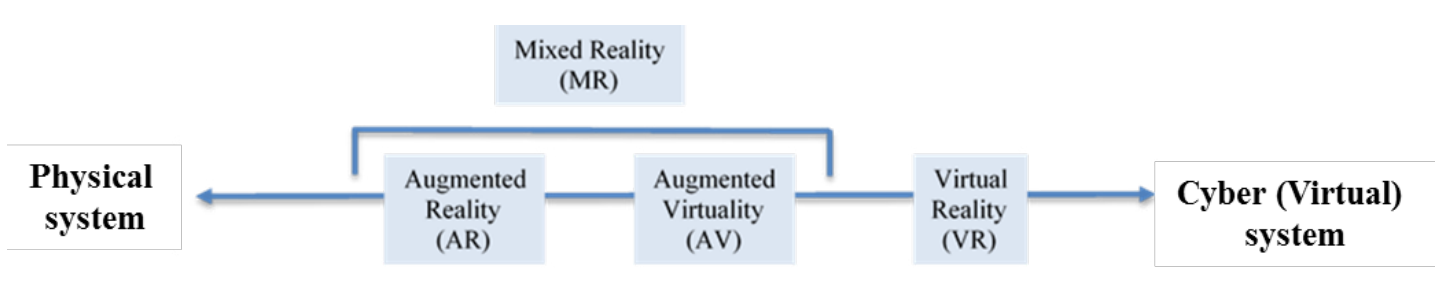
\includegraphics[width=12cm, height=3cm]{imagenes/Differences_XR_Systems.png}
\caption{Relación entre las tecnologías XR y el entorno. Fuente:\cite{Differences_XR_Systems}}
\label{fig:Differences_XR_Systems}
\end{figure}

La idea es unificarlos en un solo término conocido como realidad extendida. Para poder entender a fondo qué significa esto y como funciona, primero se debe entender bien la diferencia entre realidades virtuales, aumentadas y mixtas.

En la figura \ref{fig:XR_Introduction} se puede visualizar un objeto virtual tridimensional de un robot. Si se visualiza este robot sobre un entorno distinto al real, completamente creado por ordenador, entonces el robot está en un entorno de realidad virtual, y si se visualiza sobre el entorno real, entonces está en un entorno de realidad aumentada, tal y como se aprecia en las dos primeras representaciones. Sin embargo, estos dos conceptos pueden mezclarse, y surge como resultado la realidad mixta.

\begin{figure}[h!]
\centering
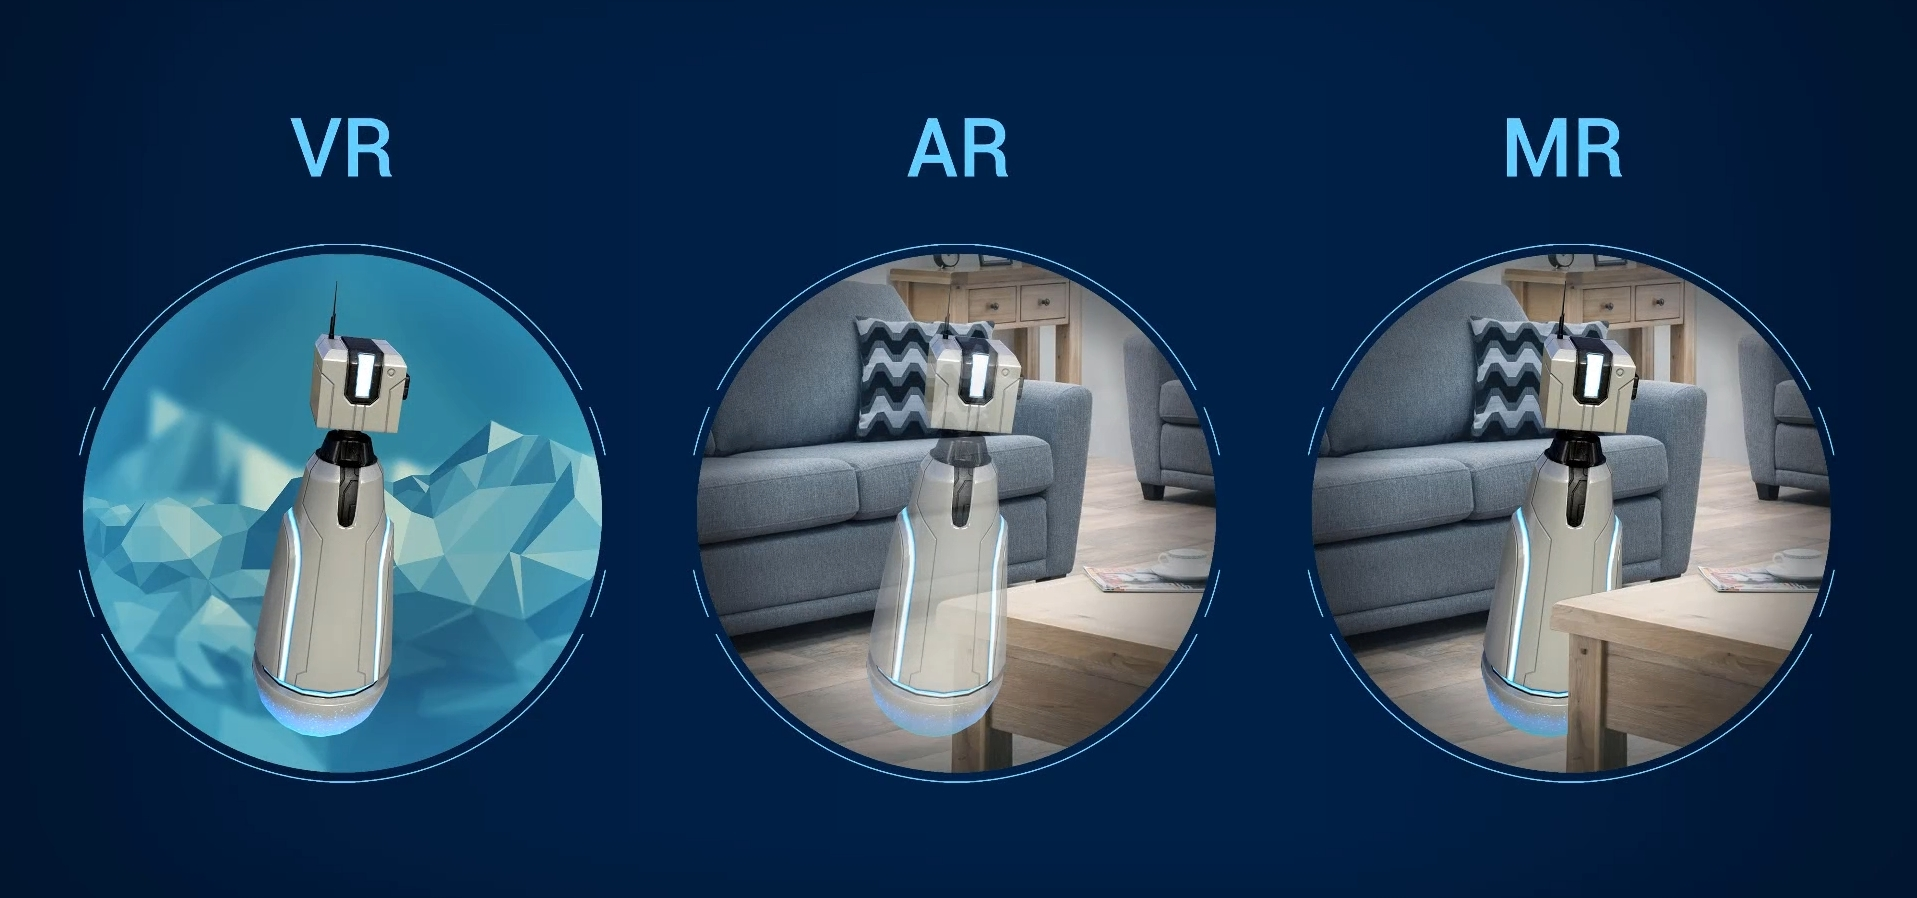
\includegraphics[width=12cm, height=6cm]{imagenes/vr_ar_mr_diffs.jpg}
\caption{Diferencias entre VR,AR y MR. Fuente:\cite{Unity_XR_Introduction}}
\label{fig:XR_Introduction}
\end{figure}

En la actualidad, la tecnología permite a los desarrolladores acceder a información sobre las diferentes profundidades de todos los objetos en un entorno real que captura una cámara, y permite que se creen interacciones entre el mundo virtual y el real. Gracias a esto se pueden conseguir efectos como situar un objeto del mundo virtual entre otros dos objetos del mundo real tal y como se muestra en la última representación de la imagen.

Esto se conoce como realidad mixta, y lo que se busca con su utilización es trasladar el mundo real a un mundo virtual, es decir, generar un entorno 3D que se adapte a la realidad y superponer información virtual de manera que se pueda añadir contenido adicional al espacio.

Una vez comprendidas las diferencias,la principal ventaja que nos proporciona utilizar este sistema es que permite desarrollar proyectos en realidad virtual para diferentes dispositivos de manera genérica, por lo que aumenta la compatibilidad. El XR Plug-in Framework permite integraciones directas desde plataformas diferentes, y está formado principalmente por una API que proporciona fun- cionalidades básicas de Unity y permite a los desarrolladores crear sus propios plug-ins e integrarlos en la plataforma, como se ve en la figura \ref{fig:XR_Architecture}.

Gracias a la arquitectura con la que se ha diseñado este sistema, si en un futuro uno o varios desarrolladores decidieran crear sus plug-ins utilizando Unity XR, hacer compatible una aplicación con ellos sería muy sencillo ya que simplemente habría que añadir sus implementaciones desde el administrador de paquetes de Unity. Esto evita hacer diferentes actualizaciones que serían necesarias para hacer funcionar aplicaciones en determinados sistemas nuevos que surgen con el tiempo.

\begin{figure}[h!]
\centering
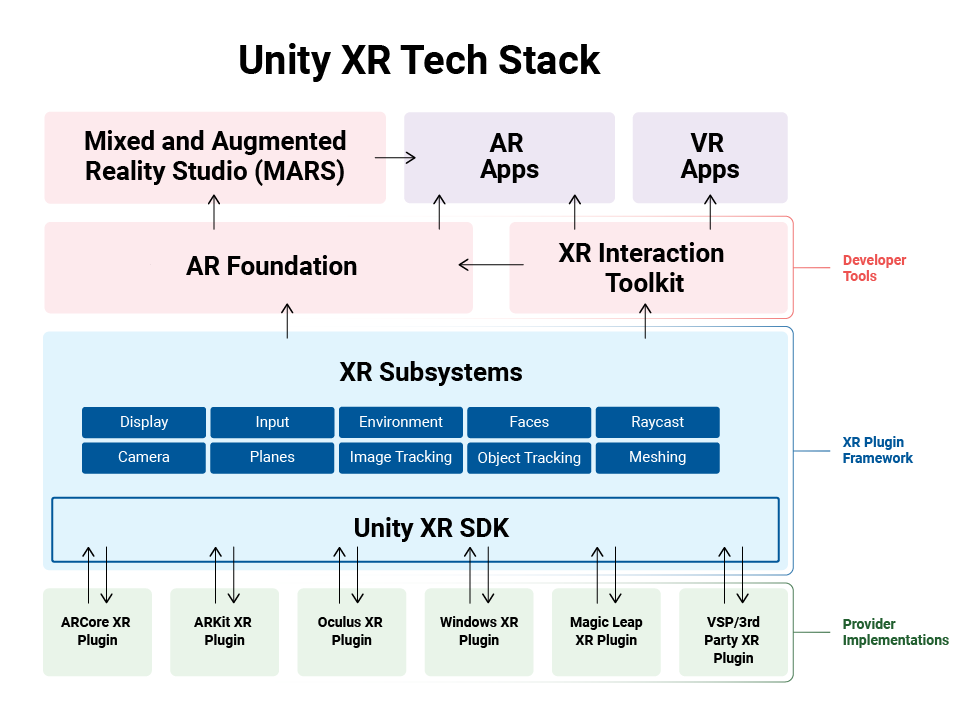
\includegraphics[width=14cm, height=10cm]{imagenes/Unity_XR_plug-in_framework.png}
\caption{Arquitectura del Unity XR Plug-in Framework. Fuente:\cite{XR_Plug-in_Framework}}
\label{fig:XR_Architecture}
\end{figure}

Por las razones enunciadas en este apartado, se utiliza este sistema para implementar la aplicación, y aumentar así la compatibilidad y disminuir problemas que podrían surgir en el futuro.

\subsection{Renderizado de objetos tridimensionales} \label{Unity_Rendering}

Uno de los aspectos claves en el desarrollo de este proyecto es el renderizado de objetos en 3D. El renderizado de un objeto  es la imágen que se crea en la escena a partir de un modelo tridimensional.

En Unity, cualquier objeto es renderizado a partir de polígonos triangulares de distintas características. Para generar estos triángulos, es necesario conocer las coordenadas de sus vértices, la orientación de su superficie y la forma en la que rebota la luz sobre ella (Ver figura \ref{fig:Unity_RenderEDA}). Con estos datos, es posible crear cualquier objeto situando los triángulos unos al lado de otros, dándoles los tamaños y características requeridos.

Para conseguir generar una figura determinada, es necesario formarla a partir de estos triángulos. Cuanto mayor sea el número de triángulos que forman la figura, mayor será su calidad ya que será más detallada y las formas triangulares serán más difíciles de percibir. Esto es de vital importancia cuando los objetos tienen formas curvas, ya que si están compuestos por pocos polígonos

\begin{figure}[h!]
\centering
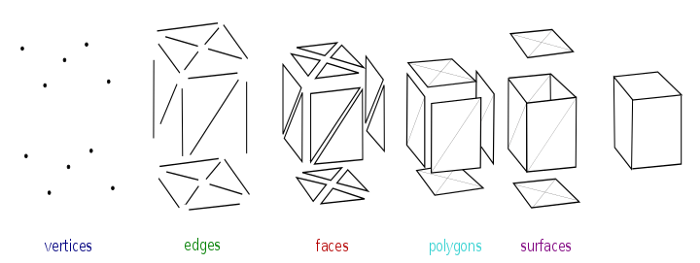
\includegraphics[width=12.5cm, height=4cm]{imagenes/Unity_Render_EDA.png}
\caption{Generación de modelos tridimensionales utilizando la información de la componente Mesh. Fuente:\cite{Unity_Render_EDA}}
\label{fig:Unity_RenderEDA}
\end{figure}

Una vez se ha generado el modelo tridimensional en la escena, hay que transformar la imagen a un plano bidimensional, ya que lo visualizamos a través de una pantalla. En este punto, es de vital importancia que la profundidad de los objetos se vea reflejada en la proyección.  

Para conseguir esto, se calculan las distancias relativas de los vértices de los objetos a la cámara y se muestran unos delante de otros según su posición, tal y como se ve en la figura \ref{fig:Unity_Projection}. 

\begin{figure}[h!]
\centering
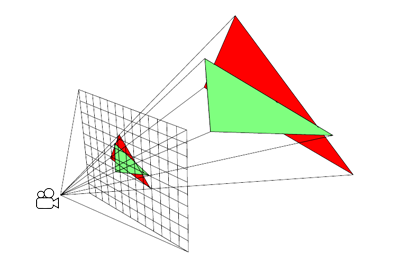
\includegraphics[width=10cm, height=7cm]{imagenes/2D_Projection_Unity.png}
\caption{Proyección de modelos 3D sobre un plano bidimensional. Fuente:\cite{Unity_Render_EDA}}
\label{fig:Unity_Projection}
\end{figure}

El principal atributo del Mesh de un objeto es el Material. Un Material define cómo se ve el objeto en la escena, es decir, su textura, color, transparencia, reflexividad de la luz... Este atributo es fundamental ya que sin él solo está definida la forma del objeto. Los Material heredan sus propiedades de los Shader, que son código que define cómo el motor gráfico tiene que renderizar el objeto \cite{Unity_Materials}. Los materiales que se utilizan pueden ser simples colores RGB, pero también se pueden utilizar texturas más complejas y personalizadas.

Una vez entendidos los Mesh y los materiales que los definen, se puede crear cualquier objeto aplicándole la textura deseada.

\section{Realidad virtual}

A lo largo de este proyecto, se utilizan dispositivos de realidad virtual para que los usuarios puedan explorar los entornos de la manera más inmersiva posible.

Como se ha mencionado anteriormente, en el desarrollo se hace uso de Unity XR, de manera que la aplicación de realidad virtual se pueda utilizar desde el mayor número de dispositivos distintos posible, con una única implementación genérica. Para que esto sea posible, estos deben dar las funcionalidades necesarias para que la aplicación pueda ejecutarse, aunque no necesariamente tienen que ser exactamente iguales entre dispositivos.

Aunque existen muchos tipos de dispositivos que tienen funcionalidades distintas, en este proyecto se utilizan los HMD  o "\uppercase{H}ead Mounted Displays" más populares, ya que son similares en muchos aspectos y proporcionan una calidad suficiente. Un HMD es, esencialmente, un casco de realidad virtual que tiene dos pantallas, una para cada ojo, de manera que, mostrando imágenes diferentes a cada ojo, las imágenes que perciben los usuarios son tridimensionales. Esta técnica se llama esteroscopía, y permite que los usuarios perciban detalles como la profundidad. También utilizan un sistema que traduce el movimiento del casco, es decir, el movimiento del usuario, gracias al sistema de cámaras y sensores integrados en el dispositivo. Esto se conoce como \textit{\uppercase{I}nside-out tracking} \cite{Inside_Out_Tracking}, y permite hacer que el usuario se sienta presente en el entorno ya que puede moverse libremente por el espacio y rotar 360º.

\subsection{Grados de libertad de movimiento}

La sensación de inmersión que tiene el usuario en los entornos virtuales es uno de los puntos más críticos en realidad virtual. 
Esta sensación depende mucho de la libertad para explorar el espacio, que está limitada por los grados de libertad o \textit{Degrees of Freedom}, de los que disponga el dispositivo que se use, y que determina los tipos de movimiento que pueden detectar.

En realidad virtual, distinguimos entre 3 y 6 grados de libertad. Con 3 grados de libertad solo se detecta rotación, es decir, el usuario puede mirar a la izquierda o a la derecha, arriba o abajo e inclinarse lateralmente. Sin embargo, si se amplían los grados de libertad a 6, los usuarios pueden también recorrer hacia delante y hacia atrás, derecha o izquierda e incluso agacharse o saltar \cite{DOF} (Ver figura \ref{fig:DOF}).

El movimiento con 3 grados de libertad es suficiente para aplicaciones en las que el usuario no tiene que moverse, si no simplemente ver el entorno, como por ejemplo una montaña rusa en realidad virtual, pero para este proyecto no es suficiente.

En general, cuanta mayor libertad de movimiento tiene el usuario, mayor es la sensación que tiene de realmente estar en el entorno virtual, y por lo tanto la experiencia que surge como resultado es más realista. Dadas estas condiciones, la respuesta más común es que el usuario actúe como lo haría en el mundo real, que es lo que la mayoría de aplicaciones de realidad virtual buscan.

%%Imagen de grados de libertad
\begin{figure}[h!]
\centering
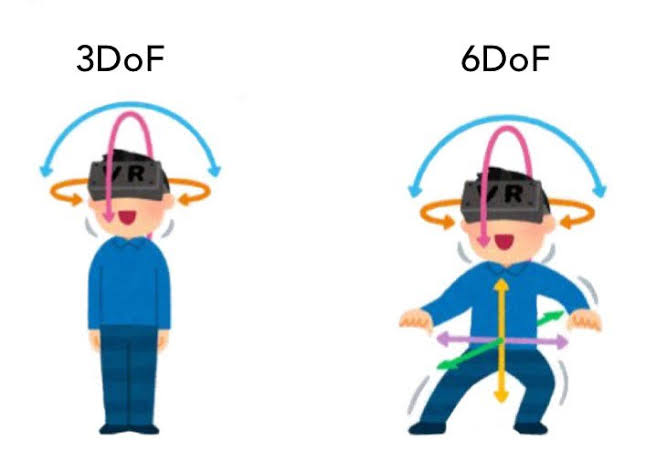
\includegraphics[width=10cm, height=6cm]{imagenes/DOF.jpg}
\caption{Diferencias entre 3 y 6 grados de libertad. Fuente:\cite{DOF_image}}
\label{fig:DOF}
\end{figure}

Como el objetivo principal de este Trabajo de Fin de Grado es poder explorar espacios infinitamente grandes utilizando entornos no euclidianos, es necesario hacer uso de dispositivos con 6 grados de libertad, ya que lo que buscamos es que el usuario no pueda hacer una distinción entre la realidad y el entorno virtual, aumentando la sensación de presencia en el entorno todo lo posible.

\subsection{Sensaciones que afectan la experiencia del usuario en entornos virtuales}
\subsubsection{Sensación de presencia}

Un entorno de realidad virtual que hace sentir al usuario que está realmente ahí, consigue una buena sensación de presencia. Esto se logra principalmente gracias a todas las funcionalidades de los dispositivos de realidad virtual, que permiten transmitir al usuario toda la información sobre el entorno y que sus sentidos la reciban de manera lo más similar posible a entornos reales. Sin embargo, también es necesario que el entorno esté construido correctamente y tenga sentido para el usuario que lo explora.

Esta sensación de presencia se busca por que prácticamente la totalidad de las aplicaciones de la realidad virtual se basan en que el usuario se comporte como lo haría en el mundo real. Tanto en aplicaciones de investigación como de entretenimiento, este factor es determinante para obtener los resultados esperados. Por ejemplo, en un juego de miedo donde se busca asustar al usuario, si el entorno estuviese muy iluminado y la música fuera alegre, el resultado probablemente no sería el que se buscaba.

Además de ayudar a conseguir buenos resultados, si el usuario se siente presente en el entorno el usuario tiende a entenderlo mejor, mapearlo y recordar los objetos que contiene.

Este hecho fue comprobado en un experimento donde se exponía a diferentes usuarios al mismo entorno virtual con dispositivos cuyos niveles de inmersión variaban \cite{Immersion_Experiment}. 

En este experimento, se diferencian 3 niveles de inmersión: bajo, medio y alto. Tras dejar que los participantes exploraran el entorno, se les propusieron diferentes preguntas sobre este. En la figura \ref{fig:Immersion_Experiment}, se pueden observar los resultados finales. Los paneles superiores muestran la precisión media de los usuarios en las preguntas, mientras que los inferiores comparan las respuestas de los participantes de cada uno de los grupos de nivel de inmersión.

\begin{figure}[h!]
\centering
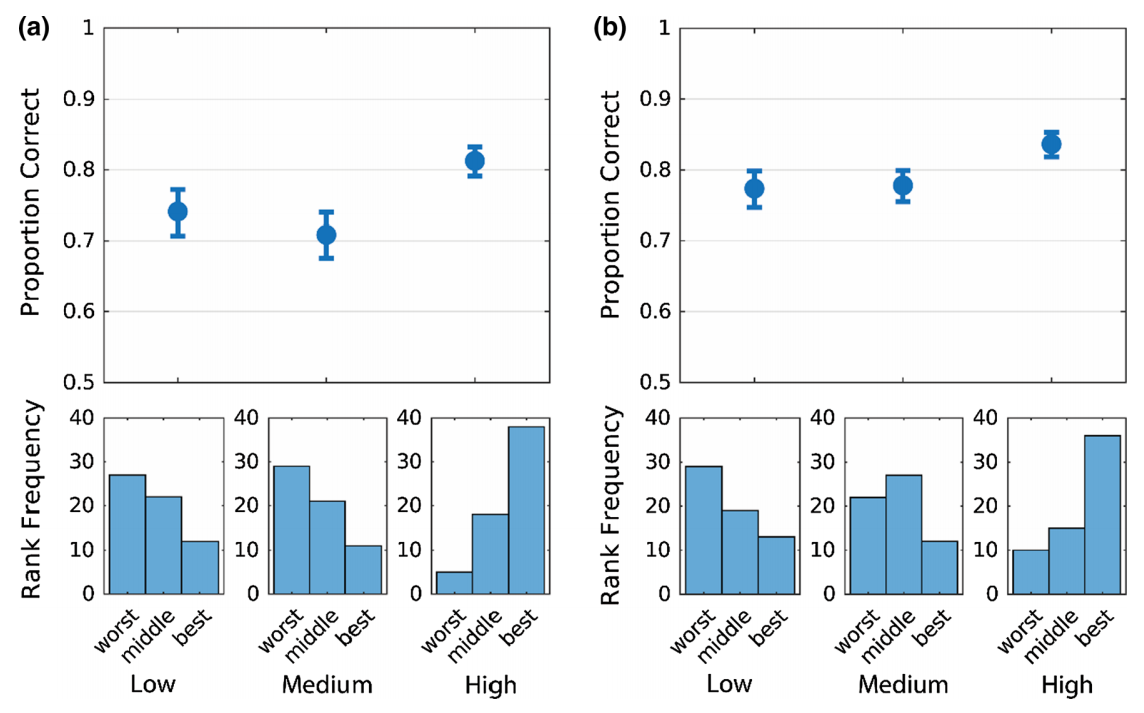
\includegraphics[height=9cm, width=13cm]{imagenes/Immersion_Experiment.png}
\caption{Contraste entre el nivel de inmersión y el rendimiento de aprendizaje de las características del entorno. a)Preguntas Si/No. b)Preguntas de respuesta múltiple. Fuente:\cite{Immersion_Experiment}}
\label{fig:Immersion_Experiment}
\end{figure}

Como se esperaba, el nivel de presencia en el entorno virtual afecta significativamente las respuestas de los usuarios, siendo los participantes del grupo de nivel de inmersión alto los que obtuvieron un número mayor de respuestas correctas. Estos resultados también muestran que los participantes cuyos dispositivos tenían un nivel de inmersión medio, en general, tenían un rendimiento menor que el resto.

Por estos motivos se concluye que cuanto mayor es la sensación de inmersión del usuario en el entorno virtual, mejores son los resultados obtenidos y la experiencia global.

\subsubsection{Cybersickness}

Aunque la presencia en el entorno virtual tiene generalmente efectos positivos, también está relacionada con otros aspectos que pueden afectar negativamente. Uno de ellos es el término cybersickness, que se refiere a las sensaciones de malestar, náuseas o mareo que percibe un usuario en un entorno de realidad virtual. Esto puede suceder en determinadas situaciones dependiendo de cada usuario.

Por ejemplo, en un simulador de conducción de vehículos algunos usuarios podrían experimentar cybersickness dadas las incoherencias entre el entorno virtual y el real. Esto ocurre por pequeños detalles como que no se siente la fuerza centrífuga al realizar un giro, o sensación de aceleración al aumentar la velocidad.

La sensación de cybersickness y de presencia están muy relacionadas de manera negativa dado que, desde una perspectiva psicológica, la magnitud del estrés en respuesta al entorno virtual se considera un indicador de presencia, y este estrés puede causar reacciones como un ritmo cardiaco elevado que aumentan las posibilidades de cybersickness \cite{Cybersickness}.

En resumen, un buen nivel de inmersión hace que los usuarios puedan entender mejor el entorno y mapearlo mentalmente, aunque dependiendo del proyecto se deben tener en cuenta otros problemas que pudiesen derivar y que podrían arruinar la experiencia como conjunto. Esta información es muy útil para el desarrollo de este proyecto ya que es completamente necesario que el usuario sienta estar en el entorno para conseguir el resultado deseado. 

\subsection{El problema del espacio de trabajo} \label{Workspace_Problem}

El espacio de trabajo disponible por los usuarios supone uno de los mayores problemas en proyectos en los que se utiliza como método de movimiento el Room Scale. Conseguir que el entorno real no suponga un límite en determinadas aplicaciones de realidad virtual supone un gran reto tecnológico que no tiene aún una solución clara.

Como se ha mencionado anteriormente, si el usuario se siente inmerso en el entorno virtual, siente que realmente está ahí, por lo que actúa como si fuese el entorno real. Esto puede ser problemático ya que los límites del espacio de trabajo siguen existiendo pese a que el usuario se olvide de ellos. Además, se debe tener en cuenta que cada usuario tiene un espacio disponible distinto, por lo que un entorno virtual que podría explorar una persona, podría salirse de los límites del espacio de trabajo de otra.

Existen algunas soluciones que permiten evitar estas posibles colisiones con objetos del mundo real. Un ejemplo serían los dispositivos Oculus, que cuentan con un sistema guardián (Ver figura \ref{fig:Sistema_Guardian}) que permite a los usuarios ver una malla tridimensional que muestra los límites del espacio de trabajo cuando el usuario se aproxima a ellos.

Estos límites son personalizables, y solo se muestran en caso de que exista peligro de salirse de ellos. Esta es una buena solución general ya que le recuerda al usuario que el entorno real sigue existiendo aunque se olvide cuando siente que está presente en el entorno virtual.

Sin embargo, este sistema no proporciona una solución completa, ya que no soluciona el problema del espacio de trabajo, sino que lo evita. Lo que se busca conseguir es que el usuario pueda recorrer cualquier parte del entorno virtual sin preocuparse del real asegurando en todo momento que esto es posible. 

\begin{figure}[h!]
\centering
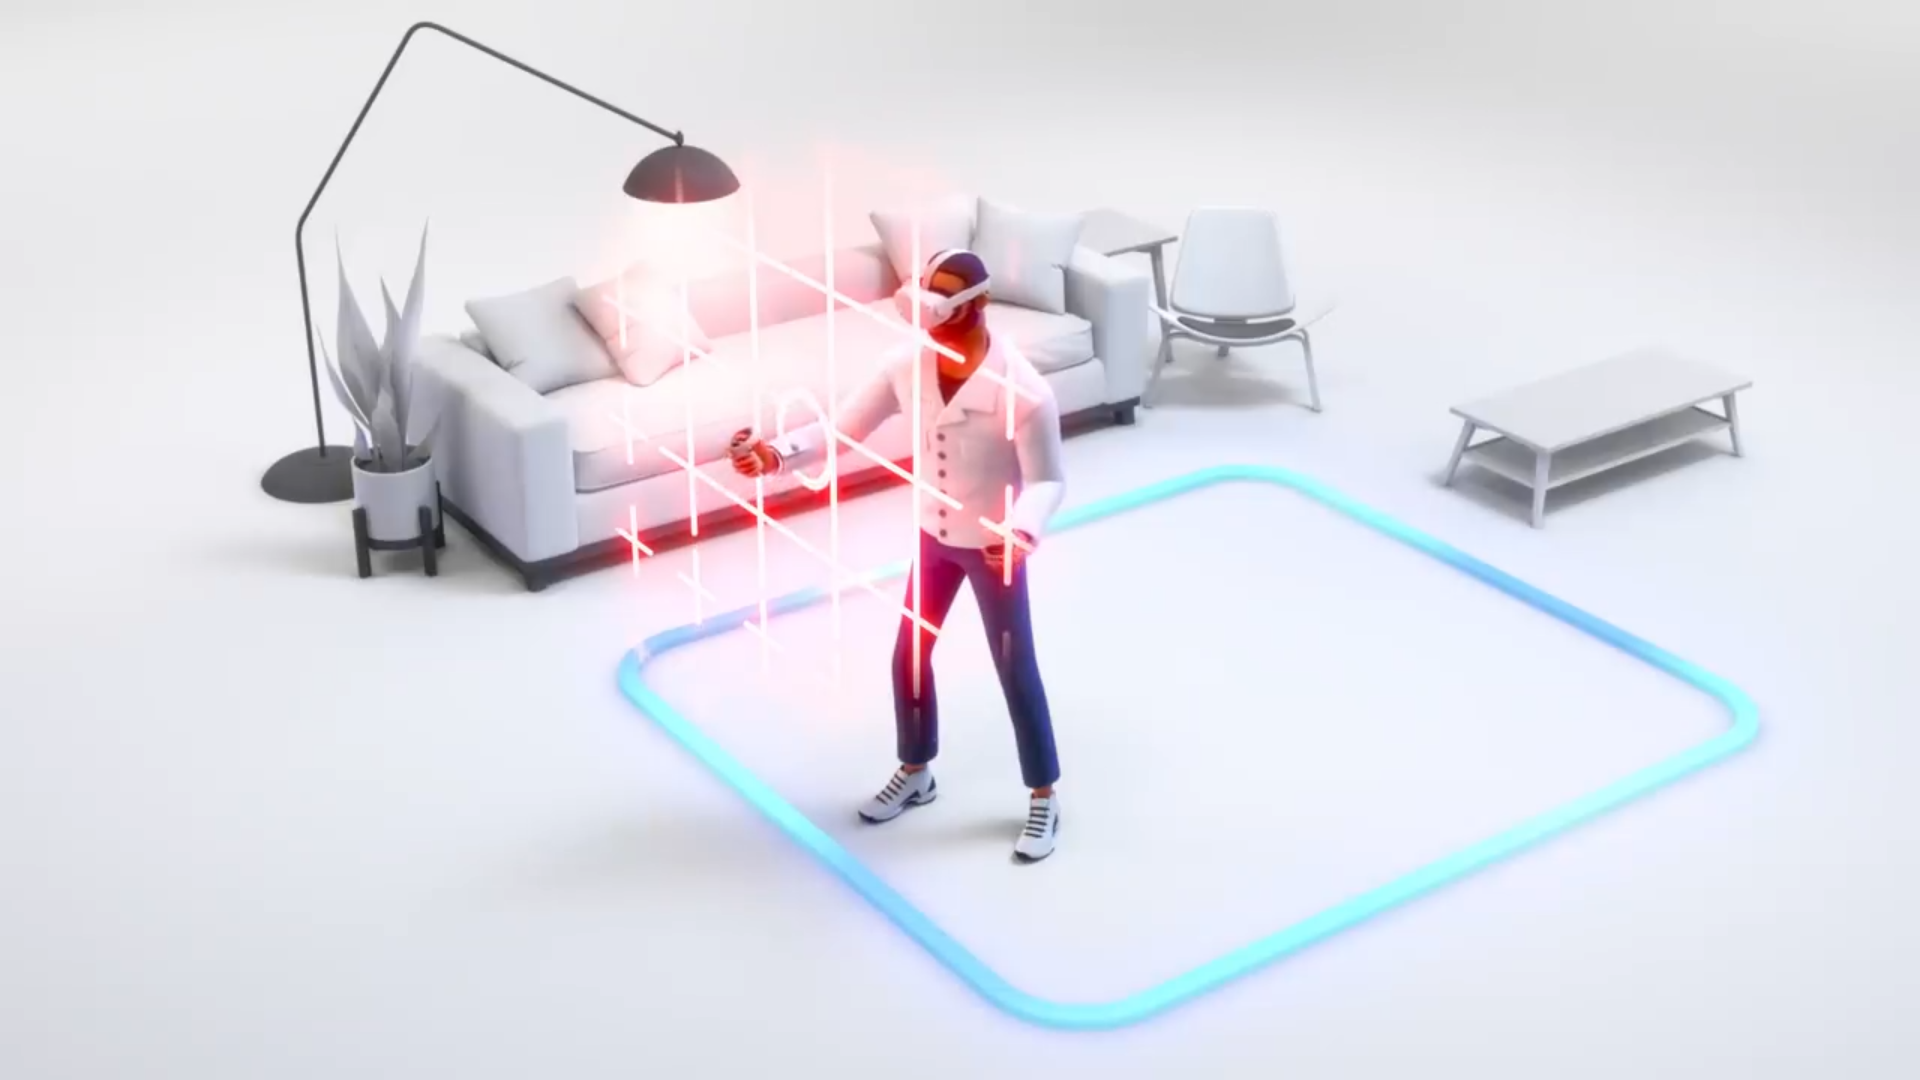
\includegraphics[height=8cm, width=12cm]{imagenes/Sistema_Guardian.png}
\caption{Sistema guardián de Oculus. Fuente:\cite{Sistema_Guardian}}
\label{fig:Sistema_Guardian}
\end{figure}

Una buena solución son los espacios no euclidianos, ya que estos permiten generar espacios infinitamente grandes en espacios limitados. El espacio disponible afecta en gran medida a las posibilidades de generación de los entornos ya que cuanto menor sea el tamaño del espacio de trabajo, menos posibilidades hay. Aun así, si se dispone de un espacio mínimo, es posible generar entornos infinitamente grandes en los que se asegure que todas las partes son explorables por el usuario.

\section{Portales en Unity} \label{Unity_Portals}
Durante el desarrollo de este Trabajo de Fin de Grado, será imprescindible la utilización del resultado que consiguió David Calderón Cortés, que desarrolló un sistema de portales en realidad virtual que nos permitirá conseguir el efecto de espacios tridimensionales no euclidianos en realidad virtual \cite{TFG_David}.

La principal funcionalidad que proporciona es conectar espacios diferentes mediante portales conectados, de manera que un usuario pueda cruzar por uno y salir por otro.

Estos portales, utilizan proyecciones tridimensionales para transformar el entorno a un plano bidimensional, de manera que podamos crear el efecto deseado. Las cámaras que capturan el entorno serán las encargadas de realizar esta transformación, de manera que sea posible crear el efecto de perspectiva, haciendo que los objetos más lejanos aparezcan más pequeños, y los más cercanos más grandes.

Al utilizar este efecto en realidad virtual, se debe hacer un buen uso de las físicas del motor gráfico ya que exponer a un usuario a cambios de gravedad o de posición bruscos puede hacer que se maree o que no entienda que está ocurriendo. Por este motivo, a diferencia de los portales del videojuego Portal, dependiendo de la orientación del portal se ajusta la gravedad de manera que el cambio sea imperceptible para el usuario. Por ejemplo, si se pasa de un portal a otro que está al revés, al cruzar se cambia el sentido en el que se ejerce la fuerza de gravedad.

Además de las físicas, hay otros aspectos de vital importancia que se tienen en cuenta para preservar la sensación de presencia. Uno de ellos es el momento exacto en el que el usuario cruza un portal, que es uno de los puntos más críticos del efecto.

%Imagen de portales hecha en photoshop
\begin{figure}[h!]
\centering
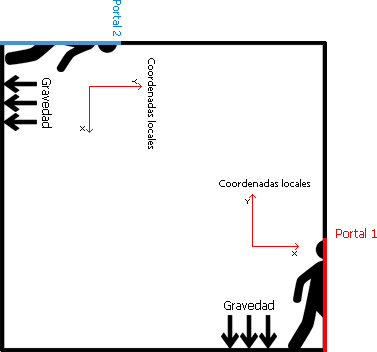
\includegraphics[width=10cm, height=9cm]{imagenes/portales.png}
\caption{Ejemplo del cambio en la gravedad cuando un usuario cruza un portal}
\label{fig:Portal_Photoshop}
\end{figure}

Como se puede ver en la figura \ref{fig:Portal_Photoshop}, tenemos un usuario que se teletransporta de un portal en una pared, a uno situado en el techo. El problema que surge es que, al salir por el portal azul, el usuario saldría con una rotación de 90º respecto a su posición original. Para solucionar esto, se debe manejar el sentido en el que actúa la gravedad para que la rotación sea imperceptible para el usuario. También hay que tener en cuenta que, al utilizar dispositivos de realidad virtual, un usuario podría cruzar un portal con un solo ojo y mantener el otro sin cruzar.

Para solucionar este último problema, se controlan las cámaras de cada ojo por separado y se utiliza un \textit{offset} muy pequeño, de manera que si uno de los ojos se acerca a esa distancia del portal se transporta al otro lado del portal, manteniendo el otro ojo sin transportar. A no ser que se sepa la existencia del efecto y se busque reproducirlo, este es imperceptible por un usuario normal.

Una vez resueltos estos problemas, el resultado es un sistema que nos permite teletransportar un usuario a cualquier punto de un espacio, de manera que para este el movimiento sea completamente natural ya que se va rotando su eje de coordenadas local y el sentido de la gravedad para compensar las rotaciones a las que se ve sometido al cruzar los diferentes portales. Así podemos conseguir que un usuario pase a caminar por las paredes o el techo sin darse cuenta de la transición.

En este proyecto haremos uso de estos portales para conectar distintas zonas del laberinto de manera que para el usuario sea imperceptible que está siendo transportado a otro lugar para conseguir el efecto de espacio no euclidiano, y que de esta manera sea posible crear un entorno infinitamente largo con un espacio de trabajo limitado.

\end{document}